\documentclass[12pt]{article}

\usepackage{fullpage}
%\usepackage[margin=0.5in]{geometry}
\usepackage{enumitem}
%\usepackage{multicol}
\usepackage{csquotes}
\usepackage{natbib}
\usepackage{tabto}
\usepackage{hyperref}
\usepackage{amsmath}
\usepackage{amssymb}
\usepackage{graphicx}

\title{Visual Motion Planning of 3-D Robots}
\author{ Avikalp Kumar Gupta \& Amitabha Mukerjee}
% \institute{Computer Science and Engineering, IIT Kanpur}

\begin{document}
\maketitle
 
\textbf{\large{Abstract}}\vspace{0.4em}\\
The aim of this project is to plan paths of multiple robots. This project is an extension of the work done by Debojyoti Das in his M. Tech. Thesis [\cite{deb}] to 3 dimensions.\\
Debojyoti developed a roadmap composition technique in multi-robot environment. The algorithm is implemented on a visual configuration space. Key traits of the algorithm:
\begin{itemize}
  \setlength\itemsep{0em}
  \item \textit{decoupled} motion planning (time efficiency)
  \item oblivious to configuration parameters (\textit{generic} method)
  \item probabilistically resolution complete
  \item Space optimality: \textit{neighbourhood product lattice} used so that Cartesian products of individual roadmaps are dynamically generated.
\end{itemize}
Debojyoti's algorithm was able to plan paths for 2-D robots. This project uses \textit{v-rep} for simulation in 3 dimensions.\\
For a particular simulation environment with $n$ cameras (vision sensors), each individual pose of the robot will be expressed as a set of $n$ images, instead of just one. This project is hence a real-world implementation of the algorithm.\\
Since, for fixed cameras, occlusion can give rise to incompleteness, hence various ways of using body-fixed cameras were being thought about as the next step in the project.

\section{Introduction}
\textit{``Traditionally, the problem has been handled using a configuration space defined in terms of \textbf{motion parameters} of the robots. An example of such motion parameters are joint angles of an articulated arm. In this work we propose a novel approach based on \textbf{visual input} alone. Such a model works on a random sample set of images of the robots without knowing the motion parameters concerned."}[\cite{deb}]\\
Even though the vision based model makes the algorithm more generic with respect to robots, it raises issues regarding the information captured. Debojyoti implemented the model for 2-D robots. In 2 dimensions, all the instantaneous information about all the objects in the environment can be captured by a single photograph. The same is not true in 3 dimensions. 

\subsection{Problem: Data Generation}
One of the problems, to begin with, is the data generation. In debojyoti's work, the images, which were used to generate the roadmaps for each robot, were generated in the following manner:
\begin{figure}
  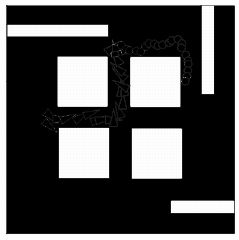
\includegraphics[width=0.5\columnwidth]{exp1_deb}
  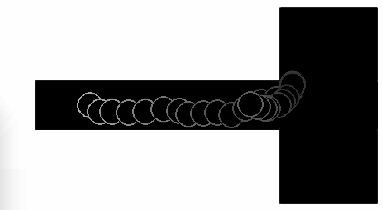
\includegraphics[width=0.5\columnwidth]{exp2_deb}
  \caption{Examples of arenas for Debojyoti's code: Black implies free area and white means obstacle. \textit{Image Source: Grayscaled (to highlight the arena) versions of images from [\cite{deb}]}}
  \label{twoD_arenas}
\end{figure}
\begin{enumerate}
  \item An image file, similar to the ones illustrated in figure \ref{twoD_arenas}, represented the arena.
  \item A position on the arena is chosen at random (and an orientation is also chosen at random) to place the robot objects.
  \item Images are validated on the basis of collision with obstacles. Hence, an image, in which any pixel of the robot coincides with any white pixel, will be rejected.
  \item Each of the remaining image represents a valid pose of the robot in consideration.
\end{enumerate}

\subsection{Problem: Image Validation}
We have to capture images of the environment using cameras and use the information from \textit{all the images} to extract information. While generating the set of valid poses, for example, if we want to check collision, we have to go through all the images: the pose is valid if there is \textit{atleast} one image in which the objects are not colliding.

But it turns out that we can never have enough (fixed) cameras. Consider the figure \ref{difficulties}. The environment, in this case, consists of 5 cameras, strategically placed at orthogonal positions to capture maximum information about the scene. The environment does not have any collision, but still all the cameras together are unable to classify this pose as valid.\\
\begin{figure}
  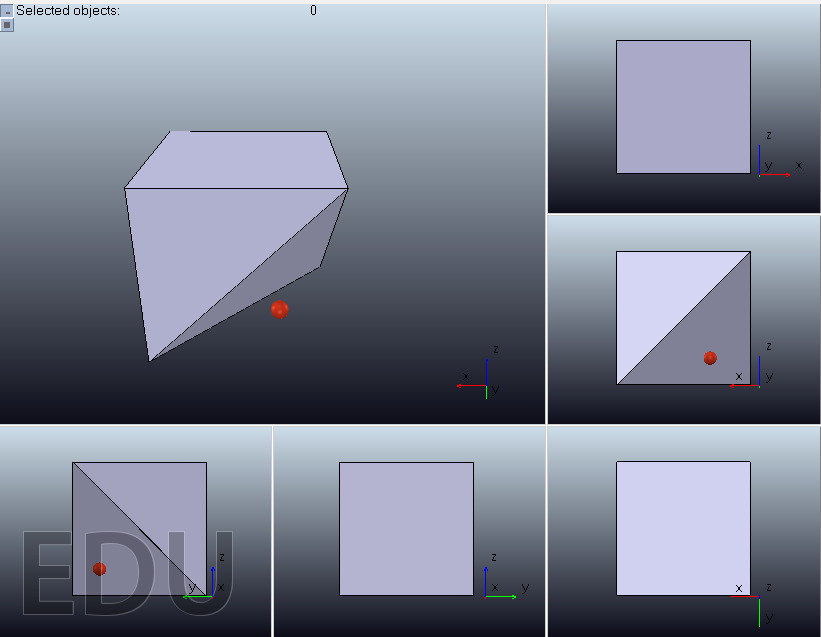
\includegraphics[width=\columnwidth]{difficulties}
  \caption{(left-top)A small sphere near a truncated cube; (others) all 5 cameras (placed at orthogonal positions) detect ``false" collision \textit{\small{(image has been generated using v-rep software)}}}
  \label{difficulties}
\end{figure}

Apart from the genericness, the paper also describes the closeness of the vision based model to humans:\\
\textit{``Human beings do not appear to use global coordinates; instead, motion is encoded (both consciously and implicitly) in terms of relative poses. Mammals navigating in familiar environments acquire ``place cells" which indicate their position in space, but these are organized in a system of neighbouring columns in the brain that encode nearby places. Thus, the representation appears to encode space in terms of nearby positions rather than a global coordinate."}[\cite{deb}]
%This motivates us to use body-fixed cameras.

\section{Idea/Approach}
The approach is similar to Debojyoti's work, which includes the following steps:
\begin{enumerate}
  \item Find a way of generating images for a particular pose of a robot from multiple cameras
  \item Create a graph using these poses (described by the set of images corresponding to the same motion parameter values)
  \item Ensure the validity of these poses, i.e. handle \textit{``static collision"}
  \item Assign weights to the edges of the graph using some metric, preferably distance between the poses
  \item Construct a road-map from the initial to the final pose (using K-nearest neighbours)
  \item Repeat the above steps for all the robots in the scene
    \item Create a composite roadmap using the roadmaps of all the robots (this includes handling \textit{``dynamic collisions"})
\end{enumerate}

%% \section{Theory}
%% \subsection{Visual Manifold Theorem}
%% In the absence of motion constraints, the pose of a mechanism with d degrees of freedom can be
%% described by a $d$-dimensional configuration vector $q$ . The space $Q$ of all possible configurations
%% is called the Configuration Space or C-space of the robot. However, how to determine $q$ is not
%% fixed; any \textit{generalized coordinate} that fully specifies the robot pose can be used. Let $R(q)$ be
%% the volume occupied by the robot in configuration $q$. $R(q)$ is a subset of $R_{sv}$ that is the volume
%% swept by the robot in all possible configurations. For a mobile robot, the degrees of freedom
%% $d = 3$, and traditionally, the configuration $q = (x, y, \theta)$ is used. We note that the topology of the
%% C-space is $\mathbb{R}^2 \times S^1$ , which is not euclidean, since as $\theta$ increases, it returns to the original pose.
%% This causes some difficulty in the algorithm, since most NLDR manifold discovery algorithms
%% (e.g. ISOMAP \cite{}) assume that the target manifold is euclidean. Now consider a camera
%% mounted on a robot that is moving in a static world. The image obtained from the camera is a
%% function of its pose q ∈ Q. The imaging transform function F () which maps a 3-D world point
%% to its image point I R = x , I R ∈ V, where V is the image space. F () is parametrized by the
%% camera imaging constants and the pose q . Under the traditional imaging situations (ignoring
%% lens distortions etc) F (q ) is a perspective transformation, which may be mapped as a linear
%% transformation in the homogeneous coordinates space.

%% Assumption (Visual distinguishability assumption).For any q 1 = q 2 , it is not the case that
%% I(q 1 ) is identical to I(q 2 ).
%% Theorem (Visual Manifold Theorem). Under visual distinguishability conditions, the parame-
%% ter space Q and the robot image space I R ⊂ V are homeomorphic.
%% Since F (q ) is linear transformation, every neighbourhood of q maps to a neighbourhood
%% on I R , that is N (q ) → N (I R ). For the other way to hold that is N (I R ) → N (q ), under the
%% assumption of “visual distinguishability”, different images must be from differing poses, so the
%% continuous image neighbourhood must be unique as well, hence the inverse also holds. Since any
%% neighbourhood has a bijective map in the other space, the parameter space Q is homeomorphic
%% to the visual space $I_R$.

%% A consequence of this theorem is that for a mobile robot camera, since the motion manifold
%% is R 2 × S 1 , the image manifold must also have the same topology.
%% In creating our visualizations below, we use these expectations to guide the data-driven
%% dimensionality reduction methods, since most NLDR methods require a target dimension to be
%% specified. Also, most NLDR methods generate euclidean topologies, and since an S 1 subspace
%% can only be mapped onto an euclidean R 2 space, this necessitates a step up in the target
%% dimension.
%% However, we note that in practice, we do not need to obtain the low dimensional embedding
%% as a set of manifold coordinates. Thus, in order to localize relative to other nearby objects, or
%% even to navigate, we do not need a set of coordinates; it is sufficient if we construct only the
%% local tangent spaces - these are done using principal component analysis on the local neighbours
%% in the images space - they correspond to charts on the manifold, and the set of all charts or the
%% atlas, is a complete representation of the manifold [4].
%% We can gain some intuition into the image manifold by noting that although images have a
%% dimensionality determined by the number of pixels, (320 × 240, say) so that each I(q ) ∈ R 80K .
%% However, assigning arbitrary colours to each of the ≈ 80K pixels will almost never generate
%% an image as seen from the mobile robot camera, hence the actual image space I R is a much
%% smaller subspace of V. In fact, what the theorem states is that the images will ideally lie on
%% a 3-dimensional manifold which is the I R subspace of V, and that it will have the topology
%% $\mathbb{R}^2 \times S^1$.

\section{Current Progress}
From the above listed steps, currently we have implemented steps 1, 2 and 3:
\begin{enumerate}
  \item : We have used \textit{v-rep software and API} to generate images [figure \ref{v-rep}].
  \item : An external python script was written using v-rep remote API which would give random values to all the joint angles of any robot present in the scene and then capture the images from each vision sensor. These images can be used to generate the road-maps.
  \item : Since v-rep only supports collision detection in its internal API, hence a work-around was figured out for this step. Motors in all joints in the environment were made immensely powerful, and instead of assigning random values to the angles, random values are assigned to the \textit{target configuration} of the joints. And this value is changed while the simulation is running. Hence the robot never reaches any impossible configuration.\\ Although, this has a drawback: the uniformity of the randomness gets reduced as the boundary configurations become more probable than the other configurations.
\end{enumerate}

\subsection{Choice of a 3-D modelling software}
\label{v-rep}
After going through some 3-D simulation softwares, we chose \textit{v-rep} over the others due to the following:
\begin{enumerate}
  \item Its free version (for educational purposes) supports most of the relevant features
  \item It is a light software and supports 3-D rendering
  \item 3-D modelling is supported inside the software, as well as 3ds-max/blender/CAD can be imported
  \item Objects and simulations can be externally controlled using its remote API for both, C/C++ and Python. (remote APIs for other languages are also supported)
  \item Proper documentation is available, and v-rep is also supported by an online forum
\end{enumerate}

\subsection{Image generation for a robot with 3 dofs (3 revolute joints)}

\begin{figure}[h]
  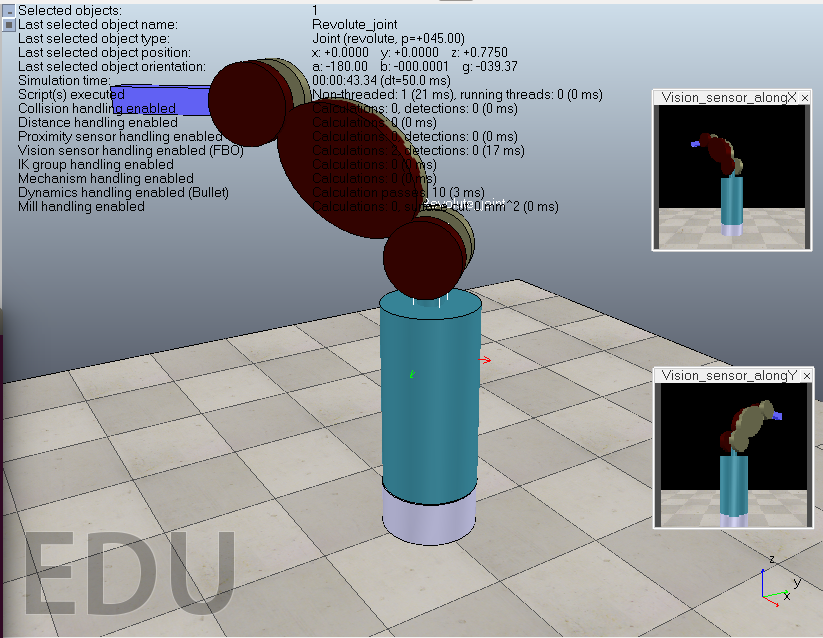
\includegraphics[width=\columnwidth]{3dof}
  \caption{Robotic arm with 3 revolute joints - Created in v-rep. The 2 smaller windows show the image captured by the 2 vision sensors installed in the scene \textit{\small{(image has been generated using v-rep software)}}}
  \label{3dof}
\end{figure}
The robot in figure \ref{3dof} was made using primitive shapes in v-rep.
It has 3 revolute joints:
One at the base, which makes whole system rotate about $z$-axis. And the other 2 have axes parallel to the $x-y$ plane.
This was created because if you consider the system installed on top of the rotating base cylinder, it is the same 2R articulate arm explained in [\cite{deb}]. Hence we have sufficient knowledge and understanding of its behaviour.

\subsection{Image generation for Baxter}
Baxter robot is one of the in-built models in v-rep.
It is a 2-armed robot with an animate face [\cite{wiki_Baxter}].
It has 3 vision sensors installed on itself, one on the head and one on each arm. Apart from this, it also has many proximity sensors on itself, which are currently irrelevant to us.
Both of baxter's arms have 7 degrees of freedom (and hence are redundant).

Apart from the robot, there are 3 other vision sensors (cameras) in the environment, one on each global axis. The images were generated for all the six cameras, but in the absence of an environment and obstacles, the images from the cameras installed on Baxter were mostly blank. The first few images from the other vision sensors are shown in figure \ref{Baxter}. You can see that they belong to the same configuration of the robot.

\begin{figure}
  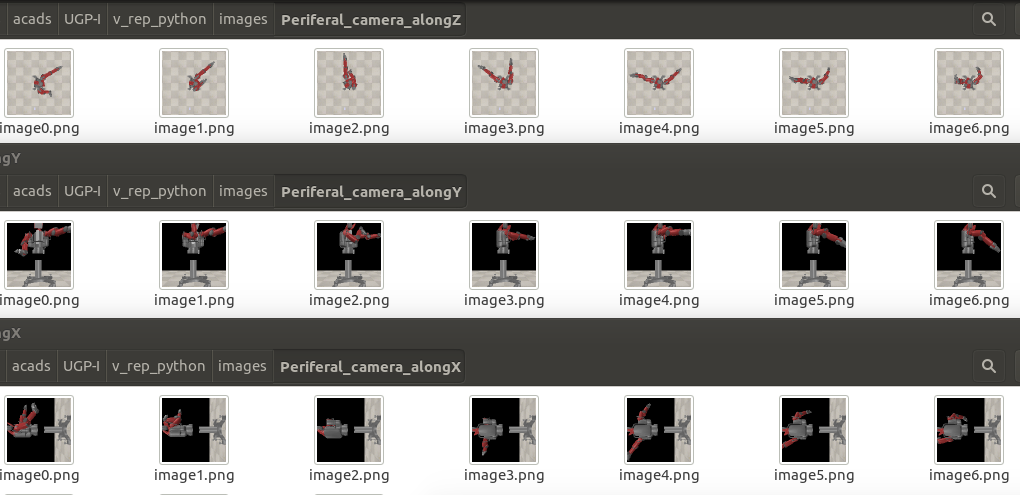
\includegraphics[width=\columnwidth]{Baxter}
  \caption{An external python script (which uses v-rep remote API) captures images from various peripheral cameras. Images with the same name belong to the same pose.}
  \label{Baxter}
\end{figure}

\section{Future Work}
For the direct extension of Debojyoti's work, the first thing to do now is to complete the remaining steps.\\ But it is quite evident that, due to occlusion, the results produced by it will not have all the traits which the planar model had. Particularly, the algorithm will not be probabilistically resolution-complete.\\
Hence, now we will proceed by understanding how humans and animals plan their motions. The implementation will be similar to paper by Amitabha Mukerjee and Divyanshu Bhartiya called ``A Visual Sense of Space" [\cite{bica}] in which they have proposed a visual characterization for the complex motions of an unknown
mobile system.

Another method could be using body-fixed cameras for capturing information about the environment (example: the case of Baxter) and making the robot learn to find the shortest path. Some study about the various neural network learning algorithms (deep learning and RNNs (including LSTMs)) was also done during the course of this project to proceed in this direction.


%\section{References}
% \bibliographystyle{unsrt}
%\bibliographystyle{alpha} 
\bibliographystyle{apalike} % AWESOME

 \bibliography{report_ref}

\section{Acknowledgement}
I would like to specially thank Mamidela Seetha Ramaiah, a.k.a. MS Ram who had shared with me some very useful libraries he had developed for processing images and generating graphs over them. He also helped me in understanding concepts related to robotics and manifolds (using Choset's book \cite{choset}).

I would also like to thank Debojyoti Das for spending some very precious time in explaining his implementation.

Lastly, I would like to thank Prof. Amitabha Mukerjee, who is the superviser of the project, for his guidance and expert advice through the project.

\end{document}
